\chapter{THz Propagation in Biological Tissue}
\label{ch:thz-propagation-biological-tissue}

\begin{nontechnical}
\textbf{What is THz radiation?} Think of it as invisible light that sits between microwaves (used in your microwave oven) and infrared (heat you feel from a fireplace). It can pass through some materials but not others.

\textbf{Why study it in tissue?} Scientists and doctors want to use THz waves to see inside skin without cutting it open---like an X-ray, but safer and better for soft tissue.

\textbf{The main challenge: Water blocks THz waves.} Your body is mostly water, and water absorbs THz radiation very strongly. This means:
\begin{itemize}
\item \textbf{Good news:} THz waves can create detailed images of skin and surface tissues
\item \textbf{Bad news:} They can't penetrate deep (only a fraction of a millimeter)
\end{itemize}

\textbf{Real-world analogy:} Imagine shining a flashlight through fog. The light gets absorbed quickly, so you can only see a short distance. THz waves in wet tissue behave the same way.

\textbf{Key takeaways:}
\begin{enumerate}
\item \textbf{THz imaging works for skin:} Doctors can detect skin cancer, assess burn depth, or check dental cavities
\item \textbf{THz cannot image deep organs:} Unlike X-rays, THz stops at the surface
\item \textbf{Safety:} THz is non-ionizing (unlike X-rays), so it doesn't damage DNA
\item \textbf{The physics:} Water molecules spin in response to THz waves, absorbing energy and turning it into heat
\end{enumerate}
\end{nontechnical}

\section{Overview}
\label{sec:thz-overview}

\textbf{Terahertz (THz) radiation} (0.1--10~THz, 30~$\mu$m--3~mm wavelength) occupies the spectral gap between microwaves and infrared. THz waves interact strongly with biological tissue due to resonances with molecular vibrations and rotations, particularly water.

\begin{keyconcept}
Understanding THz propagation is critical for three key applications:
\begin{itemize}
\item \textbf{Medical imaging:} Cancer detection, burn assessment, dental diagnostics
\item \textbf{Security screening:} Concealed weapons/explosives detection through clothing
\item \textbf{Biophysical research:} Tissue characterization and speculative neuromodulation
\end{itemize}
The primary challenge is that \textbf{water absorption dominates}, limiting penetration depth to $<$1~mm in hydrated tissue.
\end{keyconcept}

\section{Electromagnetic Properties of Biological Tissue}
\label{sec:em-properties}

\subsection{Complex Permittivity}
\label{subsec:complex-permittivity}

Biological tissue's response to EM waves is characterized by \textbf{complex relative permittivity}:
\begin{equation}
\label{eq:complex-permittivity}
\epsilon_r(\omega) = \epsilon'(\omega) - i\epsilon''(\omega)
\end{equation}
where:
\begin{itemize}
\item $\epsilon'(\omega)$ = real part (polarization, refractive index)
\item $\epsilon''(\omega)$ = imaginary part (absorption, dissipation)
\end{itemize}

\textbf{Refractive index:}
\begin{equation}
\label{eq:refractive-index}
n = \sqrt{\epsilon' \mu_r} \approx \sqrt{\epsilon'}
\end{equation}
assuming $\mu_r \approx 1$ for non-magnetic tissue.

\textbf{Absorption coefficient:}
\begin{equation}
\label{eq:absorption-coefficient}
\alpha(\omega) = \frac{\omega}{c} \sqrt{\frac{\epsilon'}{2} \left( \sqrt{1 + \left(\frac{\epsilon''}{\epsilon'}\right)^2} - 1 \right)}
\end{equation}

For low-loss materials where $\epsilon'' \ll \epsilon'$, this simplifies to:
\begin{equation}
\label{eq:absorption-simplified}
\alpha(\omega) \approx \frac{\omega \epsilon''}{2cn}
\end{equation}

\subsection{Frequency Dependence: Debye Relaxation}
\label{subsec:frequency-dependence}

\textbf{Water dominates} (tissue is $\sim$70--90\% water by mass). The \textbf{Debye relaxation model} describes water's dielectric response:
\begin{equation}
\label{eq:debye-relaxation}
\epsilon_r(\omega) = \epsilon_\infty + \frac{\epsilon_s - \epsilon_\infty}{1 + i\omega \tau}
\end{equation}
where:
\begin{itemize}
\item $\epsilon_s$ = static permittivity ($\approx$80 for water at DC)
\item $\epsilon_\infty$ = high-frequency limit ($\approx$5 for water)
\item $\tau$ = relaxation time ($\approx$8~ps for bulk water at 20°C)
\end{itemize}

\textbf{Relaxation frequency:}
\begin{equation}
\label{eq:relaxation-frequency}
f_0 = \frac{1}{2\pi \tau} \approx 20~\text{GHz}
\end{equation}

\begin{center}
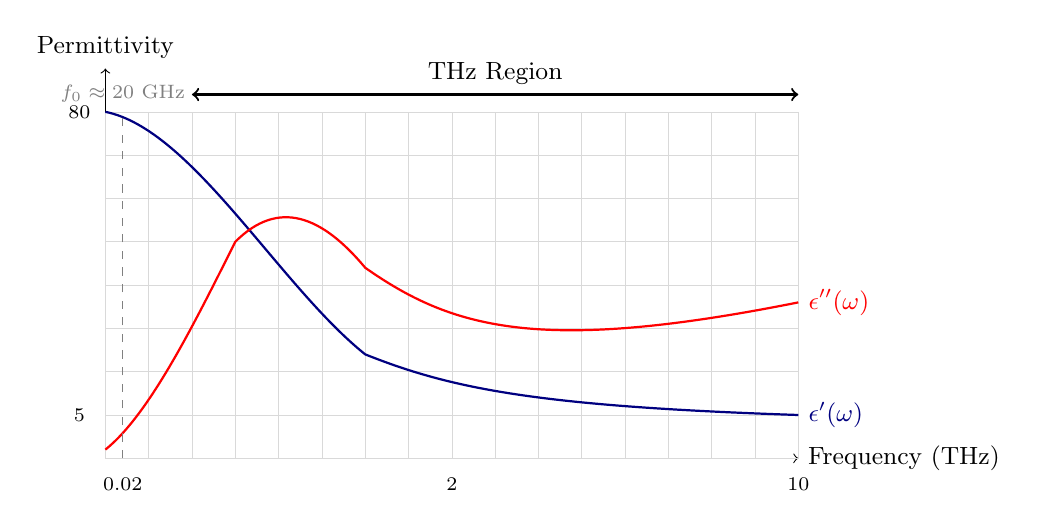
\begin{tikzpicture}[scale=1.1]
% Axes
\draw[->] (0,0) -- (8,0) node[right,font=\small] {Frequency (THz)};
\draw[->] (0,0) -- (0,4.5) node[above,font=\small] {Permittivity};

% Grid
\draw[very thin,gray!30] (0,0) grid[step=0.5] (8,4);

% Real part (epsilon')
\draw[thick,NavyBlue] (0,4) 
  .. controls (1,3.8) and (2,2) .. (3,1.2)
  .. controls (4,0.8) and (5,0.6) .. (8,0.5)
  node[right,font=\small] {$\epsilon'(\omega)$};

% Imaginary part (epsilon'')
\draw[thick,Red] (0,0.1)
  .. controls (0.5,0.5) and (1,1.5) .. (1.5,2.5)
  .. controls (2,3) and (2.5,2.8) .. (3,2.2)
  .. controls (4,1.5) and (5,1.2) .. (8,1.8)
  node[right,font=\small] {$\epsilon''(\omega)$};

% Relaxation frequency marker
\draw[dashed,gray] (0.2,0) -- (0.2,4) node[above,font=\scriptsize] {$f_0 \approx 20$ GHz};

% THz region marker
\draw[<->,thick] (1,4.2) -- (8,4.2) node[midway,above,font=\small] {THz Region};

% Labels
\node[font=\scriptsize] at (0.2,-0.3) {0.02};
\node[font=\scriptsize] at (4,-0.3) {2};
\node[font=\scriptsize] at (8,-0.3) {10};
\node[font=\scriptsize] at (-0.3,0.5) {5};
\node[font=\scriptsize] at (-0.3,4) {80};
\end{tikzpicture}
\end{center}

\textbf{At THz frequencies} (0.1--10~THz $\gg$ 20~GHz):
\begin{itemize}
\item $\epsilon'$ approaches $\epsilon_\infty \approx 5$
\item $\epsilon''$ increases linearly with frequency (Lorentzian tail)
\item \textbf{Absorption increases with frequency:} $\alpha \propto \omega \epsilon''(\omega)$
\end{itemize}

\subsection{Hydration State}
\label{subsec:hydration-state}

\textbf{Free vs bound water:}
\begin{itemize}
\item \textbf{Free water:} Bulk-like rotational dynamics, strong THz absorption
\item \textbf{Bound water:} Near protein surfaces, restricted rotation, reduced absorption
\end{itemize}

\textbf{Tissue hydration} varies significantly:

\begin{center}
\begin{tabular}{@{}lcc@{}}
\toprule
Tissue Type & Water Content & THz Absorption \\
\midrule
Skin (stratum corneum) & $\sim$20\% & Low \\
Muscle & $\sim$75\% & High \\
Fat (adipose) & $\sim$10\% & Very Low (transparent) \\
Dermis & $\sim$60\% & Moderate \\
\bottomrule
\end{tabular}
\end{center}

\begin{calloutbox}{Temperature Dependence}
Absorption increases with temperature due to faster molecular relaxation. A 10°C temperature rise can increase absorption coefficient by 15--25\%.
\end{calloutbox}

\section{Absorption Mechanisms}
\label{sec:absorption-mechanisms}

\subsection{Water Rotational Modes}
\label{subsec:water-rotational}

\textbf{Dominant mechanism:} Dipolar water molecules rotate in response to THz electric field.

\textbf{Debye absorption peak:} $\sim$20~GHz (microwave range)

\textbf{THz tail:} Absorption continues into THz due to:
\begin{itemize}
\item Hindered rotations (librational modes)
\item Collective hydrogen bond network dynamics
\end{itemize}

\textbf{Absorption coefficient} (water at 1~THz, 20°C):
\begin{equation}
\label{eq:water-absorption-1thz}
\alpha \approx 250~\text{cm}^{-1}
\end{equation}

\textbf{Penetration depth:}
\begin{equation}
\label{eq:penetration-depth-water}
\delta = \frac{1}{\alpha} \approx 40~\mu\text{m}
\end{equation}

This shallow penetration is the fundamental limitation for THz imaging in hydrated tissue!

\subsection{Protein Vibrational Modes}
\label{subsec:protein-vibrational}

\textbf{Proteins contribute} secondary absorption:
\begin{itemize}
\item \textbf{Low-frequency modes} (0.1--3~THz): Collective vibrations, domain motions
\item \textbf{Amide bands:} $\sim$6~THz (C=O stretch overtones)
\end{itemize}

\textbf{Effect:} Protein-rich tissues (e.g., collagen in dermis) have enhanced absorption at specific frequencies, providing spectroscopic contrast.

\subsection{Lipid and Membrane Absorption}
\label{subsec:lipid-membrane}

\textbf{Lipids:} Lower absorption than water/protein
\begin{itemize}
\item \textbf{Fatty acids:} CH$_2$ rocking modes at $\sim$2--4~THz
\item \textbf{Phospholipid headgroups:} Hydrated, contribute dielectric relaxation
\end{itemize}

\textbf{Cell membranes:}
\begin{itemize}
\item Thin ($\sim$7~nm lipid bilayer) $\rightarrow$ minimal direct absorption
\item But membrane-associated water has altered dynamics
\end{itemize}

\section{Scattering Mechanisms}
\label{sec:scattering-mechanisms}

\subsection{Rayleigh Scattering (Small Particles)}
\label{subsec:rayleigh-scattering}

\textbf{Condition:} Particle size $d \ll \lambda$ (THz wavelength $\sim$100~$\mu$m)

\textbf{Scattering cross-section:}
\begin{equation}
\label{eq:rayleigh-scattering}
\sigma_s \propto \left(\frac{d}{\lambda}\right)^4 \propto \omega^4
\end{equation}

\textbf{In tissue:}
\begin{itemize}
\item \textbf{Organelles} (mitochondria $\sim$1~$\mu$m, lysosomes $\sim$0.5~$\mu$m): Weak Rayleigh scattering
\item \textbf{Cellular nuclei} ($\sim$10~$\mu$m): Transition to Mie regime
\end{itemize}

\begin{keyconcept}
Scattering is weak compared to absorption at THz frequencies (unlike visible light, where scattering dominates in tissue). This is why \textbf{absorption, not scattering, limits THz penetration depth}.
\end{keyconcept}

\subsection{Mie Scattering (Comparable Size)}
\label{subsec:mie-scattering}

\textbf{Condition:} Particle size $d \approx \lambda$

\textbf{Applicable to:}
\begin{itemize}
\item Cells (10--20~$\mu$m diameter) at low THz (0.3~THz, $\lambda \approx 1000$~$\mu$m $\rightarrow$ Rayleigh regime)
\item Cells at high THz (3~THz, $\lambda \approx 100$~$\mu$m $\rightarrow$ Mie regime)
\end{itemize}

\textbf{Mie theory:} Complex calculation; depends on refractive index contrast and particle geometry.

\subsection{Interface Reflections}
\label{subsec:interface-reflections}

\textbf{Fresnel reflection} at interfaces with refractive index mismatch:
\begin{equation}
\label{eq:fresnel-reflection}
R = \left| \frac{n_1 - n_2}{n_1 + n_2} \right|^2
\end{equation}

\textbf{Tissue interfaces:}

\begin{center}
\begin{tabular}{@{}lccc@{}}
\toprule
Interface & $n_1$ & $n_2$ & Reflectance $R$ \\
\midrule
Air--skin & 1.0 & 2.2 & 15\% \\
Dermis--fat & 2.0 & 1.5 & $<$1\% \\
Tissue--bone & 2.0 & 2.5 & 20\% \\
\bottomrule
\end{tabular}
\end{center}

\begin{warningbox}
Surface reflections are significant! Impedance matching is needed for efficient THz coupling to tissue. Without it, 15\% of incident power is lost at the air-skin interface.
\end{warningbox}

\section{Penetration Depth}
\label{sec:penetration-depth}

\subsection{Beer-Lambert Law}
\label{subsec:beer-lambert}

Intensity decays exponentially:
\begin{equation}
\label{eq:beer-lambert}
I(z) = I_0 e^{-\alpha z}
\end{equation}

\textbf{Penetration depth} (1/e attenuation):
\begin{equation}
\label{eq:penetration-depth-def}
\delta = \frac{1}{\alpha}
\end{equation}

\begin{center}
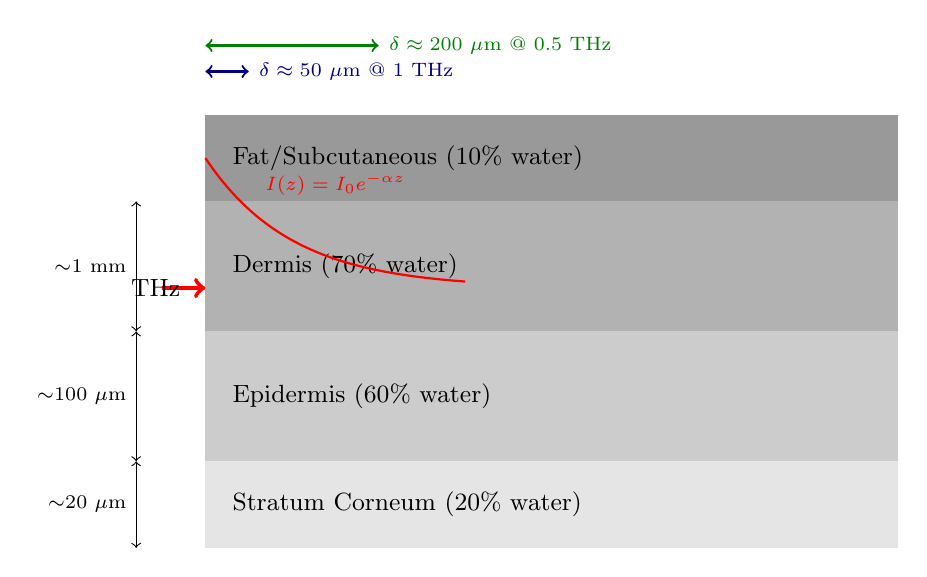
\begin{tikzpicture}[scale=1.1]
% Tissue layers
\fill[black!10] (0,0) rectangle (8,1);
\fill[black!20] (0,1) rectangle (8,2.5);
\fill[black!30] (0,2.5) rectangle (8,4);
\fill[black!40] (0,4) rectangle (8,5);

% Layer labels
\node[right,font=\small] at (0.2,0.5) {Stratum Corneum (20\% water)};
\node[right,font=\small] at (0.2,1.75) {Epidermis (60\% water)};
\node[right,font=\small] at (0.2,3.25) {Dermis (70\% water)};
\node[right,font=\small] at (0.2,4.5) {Fat/Subcutaneous (10\% water)};

% THz beam
\draw[->,ultra thick,red] (-0.5,3) -- (0,3) node[left=5pt,font=\small,text=black] {THz};

% Penetration depth markers
\draw[<->,thick,NavyBlue] (0,5.5) -- (0.5,5.5) node[right,font=\scriptsize] {$\delta \approx 50$ $\mu$m @ 1 THz};
\draw[<->,thick,Green] (0,5.8) -- (2,5.8) node[right,font=\scriptsize] {$\delta \approx 200$ $\mu$m @ 0.5 THz};

% Depth scale
\draw[<->] (-0.8,0) -- (-0.8,1) node[midway,left,font=\scriptsize] {$\sim$20 $\mu$m};
\draw[<->] (-0.8,1) -- (-0.8,2.5) node[midway,left,font=\scriptsize] {$\sim$100 $\mu$m};
\draw[<->] (-0.8,2.5) -- (-0.8,4) node[midway,left,font=\scriptsize] {$\sim$1 mm};

% Intensity decay curve
\draw[thick,red,domain=0:3,samples=100] plot (\x,{3 + 1.5*exp(-\x)});
\node[red,font=\scriptsize] at (1.5,4.2) {$I(z) = I_0 e^{-\alpha z}$};
\end{tikzpicture}
\end{center}

\subsection{Frequency Dependence}
\label{subsec:penetration-frequency}

\textbf{Typical values} (in vivo human tissue):

\begin{center}
\begin{tabular}{@{}lcc@{}}
\toprule
Frequency & Absorption ($\text{cm}^{-1}$) & Penetration depth \\
\midrule
0.1 THz & $\sim$10 & 1 mm \\
0.5 THz & $\sim$50 & 200 $\mu$m \\
1.0 THz & $\sim$200 & 50 $\mu$m \\
3.0 THz & $\sim$700 & 15 $\mu$m \\
\bottomrule
\end{tabular}
\end{center}

\begin{keyconcept}
\textbf{Key trend:} Penetration decreases rapidly with frequency. At 1~THz, THz waves barely penetrate beyond epidermis ($\sim$100~$\mu$m thick), limiting applications to \textbf{surface imaging only}.
\end{keyconcept}

\subsection{Tissue-Specific Penetration}
\label{subsec:tissue-specific}

\begin{center}
\begin{tabular}{@{}lcc@{}}
\toprule
Tissue Type & Water Content & Penetration @ 1 THz \\
\midrule
Stratum corneum & 20\% & $\sim$500 $\mu$m \\
Muscle & 75\% & $\sim$50 $\mu$m \\
Fat (adipose) & 10\% & $\sim$2 mm \\
Bone & Low (minerals) & $\sim$200 $\mu$m \\
\bottomrule
\end{tabular}
\end{center}

\begin{calloutbox}{Clinical Implication}
THz imaging is ideal for:
\begin{itemize}
\item \textbf{Skin pathology:} Basal cell carcinoma, burn assessment
\item \textbf{Surface diagnostics:} Dental caries, corneal imaging
\end{itemize}
But \textbf{poor for deep tissue imaging}---cannot image internal organs through skin.
\end{calloutbox}

\section{Wave Propagation Models}
\label{sec:propagation-models}

\subsection{Plane Wave Approximation}
\label{subsec:plane-wave}

\textbf{Assumption:} Infinite homogeneous medium

\textbf{Electric field:}
\begin{equation}
\label{eq:plane-wave}
E(z,t) = E_0 e^{-\alpha z/2} e^{i(kz - \omega t)}
\end{equation}
where $k = \omega n/c$ is the wavenumber.

\textbf{Limitations:} Ignores interfaces, scattering, finite beam effects

\subsection{Stratified Media Model}
\label{subsec:stratified-media}

\textbf{Skin structure:} Multi-layer (stratum corneum, epidermis, dermis, fat)

\textbf{Transfer matrix method:}
\begin{enumerate}
\item Divide tissue into $N$ layers
\item Apply boundary conditions at each interface (Fresnel reflection/transmission)
\item Multiply transfer matrices:
\begin{equation}
\label{eq:transfer-matrix}
\mathbf{M}_{\text{total}} = \mathbf{M}_N \cdots \mathbf{M}_2 \mathbf{M}_1
\end{equation}
\item Calculate total reflection/transmission
\end{enumerate}

\textbf{Result:} Oscillatory reflection spectrum due to interference (etalon effect in thin layers)

\subsection{Diffusion Approximation}
\label{subsec:diffusion}

\textbf{When scattering dominates} (rare in THz):
\begin{equation}
\label{eq:diffusion}
\nabla^2 U - \frac{U}{L^2} = -S
\end{equation}
where $U$ is fluence rate, $L = 1/\sqrt{3\mu_a \mu_s'}$ is diffusion length ($\mu_a$ = absorption, $\mu_s'$ = reduced scattering).

\begin{calloutbox}{Model Applicability}
The diffusion approximation is \textbf{not applicable} to most THz tissue scenarios because absorption $\gg$ scattering. Use Beer-Lambert or stratified media models instead.
\end{calloutbox}

\section{Worked Example: Penetration Depth Calculation}
\label{sec:worked-example}

\textbf{Scenario:} Calculate the penetration depth in muscle tissue at 1~THz

\subsection*{Given Parameters}

\begin{tabular}{@{}ll@{}}
Frequency & $f = 1$~THz \\
Tissue type & Muscle (75\% water) \\
Real permittivity & $\epsilon' = 9$ \\
Imaginary permittivity & $\epsilon'' = 12$ \\
\end{tabular}

\subsection*{Step 1: Calculate Refractive Index}

Using Equation~\ref{eq:refractive-index}:
\begin{equation}
n = \sqrt{\epsilon'} = \sqrt{9} = 3.0
\end{equation}

\subsection*{Step 2: Calculate Absorption Coefficient}

Using the simplified form (Equation~\ref{eq:absorption-simplified}):
\begin{equation}
\alpha = \frac{\omega \epsilon''}{2cn} = \frac{2\pi f \epsilon''}{2cn}
\end{equation}

Substituting values:
\begin{equation}
\alpha = \frac{2\pi (10^{12}) (12)}{2 (3 \times 10^{10}) (3)} = \frac{75.4 \times 10^{12}}{18 \times 10^{10}} = 419~\text{cm}^{-1}
\end{equation}

\subsection*{Step 3: Calculate Penetration Depth}

Using Equation~\ref{eq:penetration-depth-def}:
\begin{equation}
\delta = \frac{1}{\alpha} = \frac{1}{419~\text{cm}^{-1}} = 0.0024~\text{cm} = 24~\mu\text{m}
\end{equation}

\subsection*{Step 4: Calculate Power Attenuation at 100~$\mu$m}

Using Beer-Lambert law (Equation~\ref{eq:beer-lambert}):
\begin{equation}
I(100~\mu\text{m}) = I_0 e^{-\alpha z} = I_0 e^{-419 \times 0.01} = I_0 e^{-4.19} = 0.015 I_0
\end{equation}

\begin{calloutbox}[colback=black!8!white,colframe=black]{Result Summary}
At 100~$\mu$m depth in muscle tissue:
\begin{itemize}
\item \textbf{Penetration depth:} $\delta = 24$~$\mu$m
\item \textbf{Remaining power:} 1.5\% of incident (98.5\% absorbed)
\item \textbf{Implication:} THz imaging of muscle limited to very shallow depths
\end{itemize}
\end{calloutbox}

\section{Applications}
\label{sec:applications}

\subsection{Medical Imaging}
\label{subsec:medical-imaging}

\textbf{THz time-domain spectroscopy (THz-TDS):}
\begin{itemize}
\item Ultrafast THz pulse ($\sim$ps duration) transmitted/reflected from tissue
\item Time-of-flight $\rightarrow$ layer thickness
\item Spectral features $\rightarrow$ molecular composition
\end{itemize}

\noindent
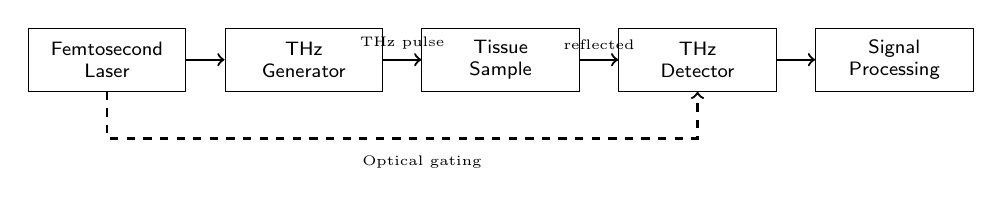
\begin{tikzpicture}[
  block/.style={rectangle, draw, minimum width=2cm, minimum height=0.8cm, font=\sffamily\scriptsize, align=center},
  node distance=1.8cm,
  font=\scriptsize
]
\node[block] (laser) {Femtosecond\\Laser};
\node[block, right of=laser, node distance=2.5cm] (gen) {THz\\Generator};
\node[block, right of=gen, node distance=2.5cm] (sample) {Tissue\\Sample};
\node[block, right of=sample, node distance=2.5cm] (det) {THz\\Detector};
\node[block, right of=det, node distance=2.5cm] (proc) {Signal\\Processing};

\draw[->,thick] (laser) -- (gen);
\draw[->,thick] (gen) -- node[above,font=\tiny] {THz pulse} (sample);
\draw[->,thick] (sample) -- node[above,font=\tiny] {reflected} (det);
\draw[->,thick] (det) -- (proc);
\draw[->,thick,dashed] (laser) |- ++(0,-1) -| (det);
\node[font=\tiny] at (4,-1.3) {Optical gating};
\end{tikzpicture}

\textbf{Clinical applications:}

\begin{center}
\begin{tabular}{@{}lp{7cm}@{}}
\toprule
Application & Diagnostic Principle \\
\midrule
Skin cancer detection & Basal cell carcinoma has altered water content $\rightarrow$ contrast \\
Burn depth assessment & Damaged tissue has different THz signature \\
Dental imaging & Caries detection (de\-min\-er\-al\-ized enamel has higher water) \\
Corneal hydration & Non-contact measurement of corneal water content \\
\bottomrule
\end{tabular}
\end{center}

\textbf{Limitations:}
\begin{itemize}
\item Shallow penetration ($<$1~mm)
\item Slow acquisition (raster scanning)
\item Requires contact or near-contact
\end{itemize}

\subsection{Security Screening}
\label{subsec:security-screening}

\textbf{Through-clothing imaging:}
\begin{itemize}
\item THz transparent to fabrics (low water)
\item Opaque to skin (high water)
\item Detect concealed weapons, explosives
\end{itemize}

\textbf{Systems:}
\begin{itemize}
\item \textbf{Passive THz cameras:} Detect natural thermal emission (3--4~THz blackbody radiation at 300~K)
\item \textbf{Active illumination:} Use THz sources for higher contrast
\end{itemize}

\textbf{Real-world deployment:}
\begin{itemize}
\item Airport security checkpoints (e.g., ProVision ATD)
\item Border crossings and high-security facilities
\item Standoff detection systems
\end{itemize}

\begin{calloutbox}{Privacy Considerations}
THz scanners can image body contours, raising ``virtual strip search'' concerns. Modern systems use privacy algorithms to obscure anatomical details while highlighting anomalies.
\end{calloutbox}

\subsection{Neuromodulation (Speculative)}
\label{subsec:neuromodulation}

\textbf{Hypothesis:} THz pulses could stimulate neurons non-invasively.

\textbf{Proposed mechanisms:}
\begin{enumerate}
\item \textbf{Thermal:} Local heating triggers temperature-sensitive ion channels (TRPV1)
\item \textbf{Non-thermal:} THz resonates with protein vibrational modes $\rightarrow$ conformational changes
\item \textbf{Quantum:} Vibronic coupling in microtubules (see Chapter on THz Resonances in Microtubules)
\end{enumerate}

\textbf{Critical challenges:}

\begin{center}
\begin{tabular}{@{}lp{7cm}@{}}
\toprule
Challenge & Issue \\
\midrule
Penetration & THz cannot reach deep brain structures transcranially (skull absorption + scalp) \\
Power & High intensity needed $\rightarrow$ thermal damage risk \\
Specificity & How to target specific neuron populations? \\
Reproducibility & Inconsistent results across studies \\
\bottomrule
\end{tabular}
\end{center}

\begin{warningbox}
\textbf{Current status:} In vitro studies show weak effects; in vivo neuromodulation has \textbf{not been convincingly demonstrated}. This remains highly speculative and requires substantial further research.
\end{warningbox}

\section{Measurement Techniques}
\label{sec:measurement-techniques}

\subsection{THz Time-Domain Spectroscopy (THz-TDS)}
\label{subsec:thz-tds}

\textbf{Setup:}
\begin{enumerate}
\item Femtosecond laser generates THz pulse via photoconductive antenna or nonlinear crystal
\item THz pulse transmitted through sample
\item Detected via electro-optic sampling (time-resolved electric field)
\end{enumerate}

\begin{center}
\begin{tabular}{@{}ll@{}}
\toprule
\multicolumn{2}{c}{\textbf{THz-TDS Characteristics}} \\
\midrule
\textbf{Advantages} & \textbf{Disadvantages} \\
\midrule
Phase-sensitive ($\epsilon'$ and $\epsilon''$) & Slow (mechanical delay line) \\
Broadband (0.1--5~THz) & Expensive (\$50k--\$200k) \\
No need for calibration standards & Requires stable environment \\
\bottomrule
\end{tabular}
\end{center}

\subsection{Continuous-Wave (CW) THz Systems}
\label{subsec:cw-thz}

\textbf{Quantum cascade lasers (QCLs):} High-power, narrow-band THz sources

\begin{center}
\begin{tabular}{@{}ll@{}}
\toprule
\textbf{Advantages} & \textbf{Disadvantages} \\
\midrule
Fast imaging & Single frequency \\
Compact & Must scan laser for spectrum \\
High power (mW level) & Limited frequency coverage \\
\bottomrule
\end{tabular}
\end{center}

\subsection{In Vivo Reflection Geometry}
\label{subsec:reflection-geometry}

\textbf{Challenge:} Most tissue measurements done in transmission; in vivo requires reflection mode.

\textbf{Reflection coefficient:}
\begin{equation}
\label{eq:reflection-coefficient}
r(\omega) = \frac{E_{\text{ref}}(\omega)}{E_{\text{inc}}(\omega)}
\end{equation}

Extract optical properties via model fitting (stratified media).

\textbf{Confounding factors:}
\begin{itemize}
\item Surface roughness
\item Sweat and moisture
\item Air gaps between probe and tissue
\item Patient motion
\end{itemize}

\section{Safety Considerations}
\label{sec:safety}

\textbf{Thermal effects:} Dominant safety concern

\textbf{ICNIRP guidelines} (International Commission on Non-Ionizing Radiation Protection):

\begin{center}
\begin{tabular}{@{}lc@{}}
\toprule
Parameter & Limit \\
\midrule
Power density & 10 mW/cm$^2$ (averaged over 6 minutes) \\
Frequency range & 0.3--3 THz \\
Temperature rise & $<$1°C for prolonged exposure \\
\bottomrule
\end{tabular}
\end{center}

\textbf{Non-thermal effects:} Controversial (see Chapter on THz Bioeffects)

\begin{keyconcept}
THz radiation is \textbf{non-ionizing} (photon energy $\sim$4~meV $\ll$ 13.6~eV ionization potential). At low intensities ($<$1~W/cm$^2$), considered safe for brief exposure.

\textbf{Key comparison:}
\begin{itemize}
\item X-rays: Ionizing, can damage DNA
\item THz: Non-ionizing, only thermal effects at normal powers
\end{itemize}
\end{keyconcept}

\section{Summary}
\label{sec:summary}

This chapter covered the fundamental physics of THz wave propagation in biological tissue:

\begin{enumerate}
\item \textbf{Complex permittivity} characterizes tissue response with real (refractive) and imaginary (absorptive) parts
\item \textbf{Water dominates absorption} via Debye relaxation, with peak at $\sim$20~GHz extending into THz
\item \textbf{Penetration depth} is limited to $<$1~mm at 1~THz due to strong water absorption
\item \textbf{Tissue-specific properties} depend on hydration state (skin vs muscle vs fat)
\item \textbf{Applications} include medical imaging, security screening, and speculative neuromodulation
\item \textbf{Safety} is generally assured at low power levels (THz is non-ionizing)
\end{enumerate}

\section{Cross-References}
\label{sec:cross-references}

\textbf{Related chapters in this book:}
\begin{itemize}
\item \textbf{Terahertz (THz) Technology} --- THz sources and detectors
\item \textbf{THz Bioeffects: Thermal and Non-Thermal} --- Biological effects of THz exposure
\item \textbf{THz Resonances in Microtubules} --- Speculative quantum effects
\item \textbf{mmWave \& THz Communications} --- Wireless applications of THz
\item \textbf{Free-Space Path Loss (FSPL)} --- Propagation fundamentals
\item \textbf{Maxwell's Equations \& Wave Propagation} --- Electromagnetic theory foundations
\end{itemize}

\section{References}
\label{sec:references}

\subsection*{Tissue Optical Properties}

\begin{enumerate}
\item \textbf{Pickwell \& Wallace}, \emph{J. Phys. D} \textbf{39}, R301 (2006) --- Comprehensive THz tissue review
\item \textbf{Smye et al.}, \emph{Phys. Med. Biol.} \textbf{46}, R101 (2001) --- Tissue dielectric properties
\end{enumerate}

\subsection*{Medical Imaging}

\begin{enumerate}
\setcounter{enumi}{2}
\item \textbf{Woodward et al.}, \emph{Phys. Med. Biol.} \textbf{47}, 3853 (2002) --- THz skin imaging
\item \textbf{Wallace et al.}, \emph{Br. J. Dermatol.} \textbf{151}, 424 (2004) --- Basal cell carcinoma detection
\end{enumerate}

\subsection*{Propagation Models}

\begin{enumerate}
\setcounter{enumi}{4}
\item \textbf{Pickwell et al.}, \emph{Appl. Phys. Lett.} \textbf{84}, 2190 (2004) --- Stratified media modeling
\end{enumerate}

\subsection*{Safety}

\begin{enumerate}
\setcounter{enumi}{5}
\item \textbf{ICNIRP}, \emph{Health Phys.} \textbf{99}, 818 (2010) --- THz exposure guidelines
\end{enumerate}
